% Copyright 2004 by Till Tantau <tantau@users.sourceforge.net>.
%
% In principle, this file can be redistributed and/or modified under
% the terms of the GNU Public License, version 2.
%
% However, this file is supposed to be a template to be modified
% for your own needs. For this reason, if you use this file as a
% template and not specifically distribute it as part of a another
% package/program, I grant the extra permission to freely copy and
% modify this file as you see fit and even to delete this copyright
% notice. 

\documentclass[10pt, mathserif, profesionalfont]{beamer}

\usepackage[utf8]{inputenc}
\usepackage[spanish]{babel}



\usepackage{amsmath,amsfonts,amssymb,amsthm}
\usepackage{booktabs}
\usepackage{hyperref}
\usepackage{authblk}

\usepackage[acronym]{glossaries}

\renewcommand\Affilfont{\itshape\small}
\renewcommand\Authand{ y }

\newtheorem{thm}{Teorema}

\usepackage{array}
\newcolumntype{L}[1]{>{\raggedright\let\newline\\\arraybackslash\hspace{0pt}}p{#1}}
\newcolumntype{C}[1]{>{\centering\let\newline\\\arraybackslash\hspace{0pt}}p{#1}}
\newcolumntype{R}[1]{>{\raggedleft\let\newline\\\arraybackslash\hspace{0pt}}p{#1}}

\newcolumntype{X}[1]{>{\raggedright\let\newline\\\arraybackslash\hspace{0pt}}m{#1}}
\newcolumntype{Y}[1]{>{\centering\let\newline\\\arraybackslash\hspace{0pt}}m{#1}}
\newcolumntype{Z}[1]{>{\raggedleft\let\newline\\\arraybackslash\hspace{0pt}}m{#1}}

\usepackage{color}
\makeglossaries

\newacronym{ndtm}{NDTM}{Máquina de Turing No Determinista}

\newacronym{sat}{SAT}{SATISFACTIBILIDAD}

\newacronym{3sat}{3SAT}{3-SATISFACTIBILIDAD}
\usepackage{float}
\usepackage{graphicx}
\graphicspath{{img/}}


% There are many different themes available for Beamer. A comprehensive
% list with examples is given here:
% http://deic.uab.es/~iblanes/beamer_gallery/index_by_theme.html
% You can uncomment the themes below if you would like to use a different
% one:
%\usetheme{AnnArbor}
%\usetheme{Antibes}
%\usetheme{Bergen}
%\usetheme{Berkeley}
%\usetheme{Berlin}
%\usetheme{Boadilla}
%\usetheme{boxes}
\usetheme{CambridgeUS}
%\usetheme{Copenhagen}
%\usetheme{Darmstadt}
%\usetheme{default}
%\usetheme{Frankfurt}
%\usetheme{Goettingen}
%\usetheme{Hannover}
%\usetheme{Ilmenau}
%\usetheme{JuanLesPins}
%\usetheme{Luebeck}
%\usetheme{Madrid}
%\usetheme{Malmoe}
%\usetheme{Marburg}
%\usetheme{Montpellier}
%\usetheme{PaloAlto}
%\usetheme{Pittsburgh}
%\usetheme{Rochester}
%\usetheme{Singapore}
%\usetheme{Szeged}
%\usetheme{Warsaw}

\title{PARTITION}

% A subtitle is optional and this may be deleted
\subtitle{Seis problemas básicos $\mathcal{NP}$-completos}

\author{David Pérez Rivero \and Alejandro Marrero Díaz}
% - Give the names in the same order as the appear in the paper.
% - Use the \inst{?} command only if the authors have different
%   affiliation.

\institute[ULL]{Universidad de La Laguna} % (optional, but mostly needed)

% - Use the \inst command only if there are several affiliations.
% - Keep it simple, no one is interested in your street address.

\date{Curso 2016/2017}
% - Either use conference name or its abbreviation.
% - Not really informative to the audience, more for people (including
%   yourself) who are reading the slides online

\subject{Theoretical Computer Science}
% This is only inserted into the PDF information catalog. Can be left
% out. 

% If you have a file called "university-logo-filename.xxx", where xxx
% is a graphic format that can be processed by latex or pdflatex,
% resp., then you can add a logo as follows:

% \pgfdeclareimage[height=0.5cm]{university-logo}{university-logo-filename}
% \logo{\pgfuseimage{university-logo}}

% Delete this, if you do not want the table of contents to pop up at
% the beginning of each subsection:
\AtBeginSubsection[]
{
  \begin{frame}<beamer>{Outline}
    \tableofcontents[currentsection,currentsubsection]
  \end{frame}
}

% Let's get started
\begin{document}

\begin{frame}
  \titlepage
\end{frame}



\section{Introduction}


\begin{frame}{Problemas involucrados}
    
\begin{block}{\gls{3dm}}
{\small 
\noindent ENTRADA: Sea el conjunto T y un entero k.

\noindent PREGUNTA: ¿Existe un emparejamiento tridimensional M $\subseteq$ T con $\mid$M$\mid$ $\geq$ k? 
}
\end{block}

\end{frame}


\section{Demostración de NP-completitud}

\begin{frame}{Partition es NP-completo I}
    
\begin{block}{Partition $\in \mathcal{NP}$}    
Es fácil comprobar que \gls{part}	$\in \mathcal{NP}$, ya que se puede encontrar una algoritmo para una \gls{ndtm} que reconozca el lenguaje $L(\mbox{part},e)$, para un esquema de codificación $e$, en un número de pasos acotado por una función polinomial.

\end{block}

\end{frame}

\begin{frame}{Partition es NP-completo II}
    
\begin{block}{Partition $\in \mathcal{NP}$}   
Sólo necesita un subconjunto A' de A y comprobar que la suma de los tamaños de los elementos en A' es la misma que para los elementos de A-A'.
\end{block}

\begin{block}{} 
Transformaremos $\gls{3dm}\rightarrow\gls{part}$ 
\end{block}

\end{frame}


\begin{frame}{Partition es NP-completo III}

\begin{block}{Partition $\alpha$ 3DM}    
Sean los conjuntos W, X, Y tal que \(\mid W\mid = \mid X\mid = \mid Y\mid = q\) 
\end{block}

\begin{block}{}
Y además que cumpla \(M\subseteq W x X x Y\) como una instancia arbitraria del \gls{3dm}, donde \(k = \mid M\mid\) 
\end{block}

\begin{block}{}
Construimos un conjunto A con tamaña $s(a)\in Z^+$ para cada $a\in A$ de forma que A contiene un subconjunto A' que satisface
\[\sum_{a \in A'}^{} s(a) = \sum_{a \in A-A'}^{} s(a)\]
\end{block}


\end{frame}

\begin{frame}{Partition es NP-completo IV}
    
\begin{block}{Partition $\alpha$ 3DM}    
El conjunto A debe contener un total de $k+2$ elementos y será construido en dos pasos.
Los primeros \textit{k} elementos de A son ${a_i:1\leq i\leq k}$, donde el elemento $a_i$ esta asociado con una tripleta $m_i\in M$.
\end{block}
\begin{block}{}
El tamaño $s(a_i)$ de $a_i$ será especificado dando su representación binaria, en términos de una cadena de 0's y 1's dividida en 3q "zonas" de \(p= \ceil \lg (k+1) \ceil\) bits cada una
\end{block}
\end{frame}

\begin{frame}{Partition es NP-completo V}
    
\begin{block}{Partition $\alpha$ 3DM}    
\begin{figure}[H]
    \centering
    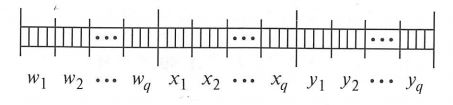
\includegraphics{figura1}
\end{figure}

\end{block}

\end{frame}


\begin{frame}{Partition es NP-completo VI}
\begin{block}{Partition $\alpha$ 3DM}    
Dado que cada $s(a_i)$ puede ser representado como un número binario con no más de \textit{3pq} bits, esta claro que $s(a_i)$ puede ser construido desde la instancia 3DM en tiempo polinomial. 
\end{block}
\begin{block}{}
Lo importante es observar en esta parte de la construcción es que, si sumamos todas las entradas de cada zonas, para todos los elementos \({a_i:\leg i\leq k}\), el total nunca superará \(k=2^p-1\). 
\end{block}
\end{frame}


\begin{frame}{Partition es NP-completo VII}
    
\begin{block}{Partition $\alpha$ 3DMT}    
Por lo tanto, al sumar \(\sum_{a \in A'}^{} s(a)\) para cada subconjunto \(A'\subseteq\{a_i:\leg i\leq k\}\) satisfará
\[\sum_{a \in A'}^{} s(a) = B\]
\end{block}

\begin{block}{}
Sí y sólo sí \(M' = \{m_i:a_i \in A'\}\) es un emparejamiento para M.
\end{block}
\end{frame}



\begin{frame}{Partition es NP-completo VIII}
    
\begin{block}{Partition $\alpha$ 3DM}    
El paso final de la construcción denota los dos últimos elementos de A como $b_1$ y $b_2$ con tamaño:
\[s(b_1) = 2 \Big[\sum_{i=1}^{k} s(a_i)\Big] - B\]

\[s(b_1) = 2 \Big[\sum_{i=1}^{k} s(a_i)\Big] + B\]
\end{block}

\end{frame}

\begin{frame}{Partition es NP-completo IX}
    
\begin{block}{Partition $\alpha$ 3DM}    
Representadas en binario con no más de $3pq + 1$ bits $\rightarrow$ construidas así en tiempo polinomial en el tamaño de la instancia dada del problema \gls{3dm}.
\end{block}

\end{frame}



\begin{frame}{Partition es NP-completo X}
    
\begin{block}{Partition $\alpha$ 3DM}    
Si suponemos un subconjunto $A' \subseteq A$ tal que
\[\sum_{a \in A'}^{} s(a) = \sum_{a \in A-A'}^{} s(a)\]
\end{block}
\begin{block}{}
\(2\sum_{i=1}^{k} s(a_i)\), y uno de los dos conjuntos, A' o A-A', contiene $b_1$ pero no $b_2$.
\end{block}
\end{frame}


\begin{frame}{Partition es NP-completo XI}
    
\begin{block}{Partition $\alpha$ 3DM}  
Al contrario, si \(M'\subseteq M\) es un emparejamiento, entonces el conjunto \(\{b_1\} \cup \{a_i:m_i\in M'\}\) forma el deseado conjunto A' para la instancia de \gls{part}. \par
\end{block}

\begin{block}{}
Por lo tanto, \(\gls{3dm} \alpha \gls{part}\), y se prueba así la $\mathcal{NP}$-completitud.
\end{block}
\end{frame}


\end{document}


